\documentclass[12pt]{article}

\usepackage{graphicx}
\usepackage{paralist}
\usepackage{amsfonts}
\usepackage{amsmath}
\usepackage{hhline}
\usepackage{booktabs}
\usepackage{multirow}
\usepackage{multicol}
\usepackage{url}

\oddsidemargin -10mm
\evensidemargin -10mm
\textwidth 160mm
\textheight 200mm
\renewcommand\baselinestretch{1.0}

\pagestyle {plain}
\pagenumbering{arabic}

\newcounter{stepnum}

%% Comments

\usepackage{color}

\newif\ifcomments\commentstrue

\ifcomments
\newcommand{\authornote}[3]{\textcolor{#1}{[#3 ---#2]}}
\newcommand{\todo}[1]{\textcolor{red}{[TODO: #1]}}
\else
\newcommand{\authornote}[3]{}
\newcommand{\todo}[1]{}
\fi

\newcommand{\wss}[1]{\authornote{blue}{SS}{#1}}

\title{Assignment 4, Design Specification}
\author{SFWRENG 2AA4}

\begin{document}

\maketitle
This Module Interface Specification (MIS) document contains modules, types and
methods for implementing the game \textit{2048}. 2048 is often played on a plain 4×4 grid, with numbered tiles that slide when a player moves them using the four arrow keys.
Every turn, a new tile randomly appears in an empty spot on the board with a value of either 2 or 4. 
Tiles slide as far as possible in the chosen direction until they are stopped by either another tile or the edge of the grid. If two tiles of the same number collide while moving, they will merge into a tile with the total value of the two tiles that collided.
The resulting tile cannot merge with another tile again in the same move.  The 
game can be launched and play by typing \texttt{make demo} in terminal.
\\\\
reference:https://en.wikipedia.org/wiki/2048_(video_game)


\newpage

\section{Overview of the design}

This design applies Module View Specification (MVC) design pattern, Strategy design pattern and Singleton design pattern. The MVC components
are \textit{GameController} (controller module), \textit{BoardT} (model module), and \textit{UserInterface} (view module).
\bigskip

\noindent An UML diagram is provided below for visualizing the structure of this software architecture

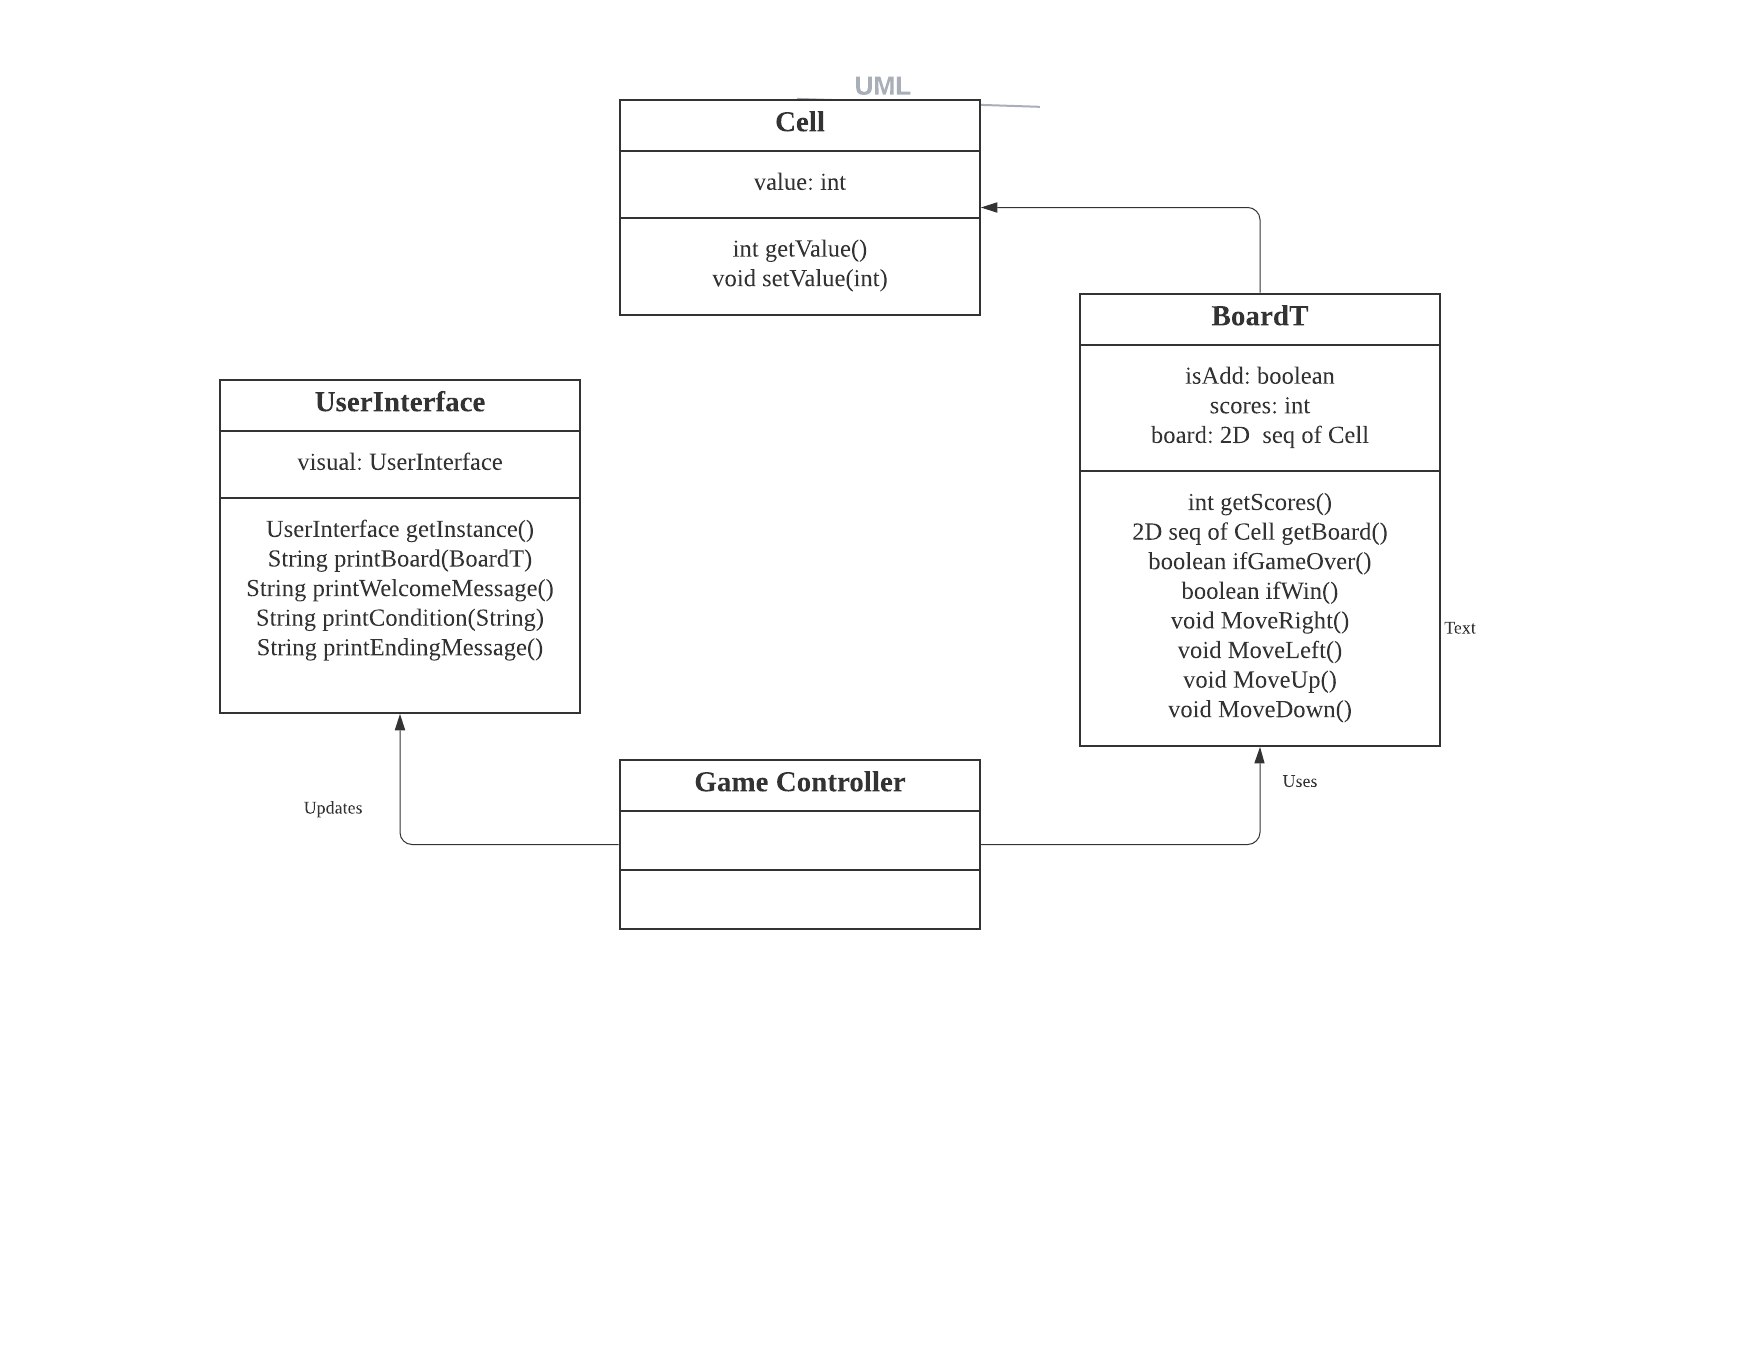
\includegraphics[width=0.9\textwidth]{UML.png}

\medskip
The MVC design pattern is specified and implemented in the following way: the module \textit{BoardT}
stores the state of the game board and the status of the game. A view module \textit{UserInterface} can display
the state of the game board and game using a text-based graphics. The controller \textit{GameController}
is responsible for handling input actions. 

\medskip

For \textit{GameController} and \textit{UserInterface}, use the getInstance() method to obtain the abstract object.

\newpage

\subsection*{Likely Changes my design considers:}

\begin{itemize}
  \item Data structure used for storing the game board
  \item The visual representation of the game such as UI layout. 
  \item Change in peripheral devices for taking user input. 
  \item Change in game ending conditions to adjust the difficulty of the game.
  \item Design more modes to have more fun such as set a timer. 
\end{itemize}

\newpage

\section* {Cell Module}

\subsection*{Module}

Cell

\subsection* {Uses}

N/A

\subsection* {Syntax}

\subsubsection* {Exported Constants}

None

\subsubsection* {Exported Types}

None

\subsubsection* {Exported Access Programs}

\begin{tabular}{| l | l | l | l |}
  \hline
  \textbf{Routine name} & \textbf{In} & \textbf{Out} & \textbf{Exceptions}\\
  \hline
  Cell & $\mathbb{N}$ & Cell & IllegalArgumentException\\
  \hline
  getValue & ~ & $\mathbb{N}$ & \\
  \hline
  setValue & $\mathbb{N}$ & Cell & IllegalArgumentException\\
  \hline
  \end{tabular}

\subsection* {Semantics}

\subsubsection* {State Variables}

value: $\mathbb{N}$

\subsubsection* {State Invariant}

None

\subsubsection* {Access Routine Semantics}

Cell(v):
\begin{itemize}
\item transition: value $:=$ $v$
\item output: $out := \mathit{self}$
\item exception: $exc :=$ ($\neg (v = 0 || v = 2 || v = 4 || v = 8 || v = 16 || v = 32 || v = 64 || v = 128 || v = 256 || v = 512 || v = 1024 || v = 2048) \Rightarrow IllegalArgumentException$)
\end{itemize}

\noindent getValue():
\begin{itemize}
\item transition: None
\item output: $out :=$ value
\item exception: None
\end{itemize}

\noindent setValue():
\begin{itemize}
\item transition: value $:=$ $v$
\item output: None
\item exception: $exc :=$ ($\neg (v = 0 || v = 2 || v = 4 || v = 8 || v = 16 || v = 32 || v = 64 || v = 128 || v = 256 || v = 512 || v = 1024 || v = 2048) \Rightarrow IllegalArgumentException$)
\end{itemize}

\newpage

\section* {Board ADT Module}

\subsection*{Template Module inherits EndCondition}

BoardT 

\subsection* {Uses}

Cell

\subsection* {Syntax}

\subsubsection* {Exported Types}

None

\subsubsection* {Exported Constant}

None

\subsubsection* {Exported Access Programs}

\begin{tabular}{| l | l | l | l |}
\hline
\textbf{Routine name} & \textbf{In} & \textbf{Out} & \textbf{Exceptions}\\
\hline
BoardT & ~ & BoardT & \\
\hline
getScores & ~ & $\mathbb{N}$ & \\
\hline
getBoard & ~ & seq of (seq of Cell) & \\
\hline
ifGameOver & ~ & $\mathbb{B}$ & \\
\hline
ifWin & ~ & $\mathbb{B}$ & \\
\hline
MoveRight & ~ & BoardT & \\
\hline
MoveLeft & ~ & BoardT & \\
\hline
MoveUp & ~ & BoardT & \\
\hline
MoveDown & ~ & BoardT & \\
\hline
\end{tabular}

\subsection* {Semantics}

\subsubsection* {State Variables}

board: sequence of (sequence of Cell) \\
isAdd: $\mathbb{B}$ \\
scores: $\mathbb{N}$

\subsubsection* {State Invariant}

None

\subsubsection* {Assumptions}

\begin{itemize}
  \item The constructor BoardT is called for each object instance before any other access
  routine is called for that object.
\end{itemize}

\subsubsection* {Access Routine Semantics}

BoardT():
\begin{itemize}
\item transition: \\
      board $:=$ 
      ($\langle \begin{array}{c}
      \langle \mbox{Cell(0)}_0, ... ... ,\mbox{Cell(0)}_3 \rangle\\
      \langle \mbox{Cell(0)}_0, ... ... ,\mbox{Cell(0)}_3 \rangle\\
      \langle \mbox{Cell(0)}_0, ... ... ,\mbox{Cell(0)}_3 \rangle\\
      \langle \mbox{Cell(0)}_0, ... ... ,\mbox{Cell(0)}_3 \rangle\\
      \end{array} \rangle$ \Rightarrow createNew() \Rightarrow createNew()) \\ 
      isAdd, scores $=$ true, 0
\item output: $out := \mathit{self}$
\item exception: none
\end{itemize}

\noindent getScores():
\begin{itemize}
\item transition: none
\item output: $out :=$ scores
\item exception: none
\end{itemize}

\noindent getBoard():
\begin{itemize}
\item transition: none
\item output: $out :=$ board
\item exception: none
\end{itemize}

\noindent ifGameOver():
\begin{itemize}
\item transition: none
\item output: true if values for all Cell in board are not zero and there is no cell whose value is as same as its left Cell or its right Cell or its unpper Cell or its lower Cell. 
\item exception: none
\end{itemize}

\noindent ifWin($x, y$):
\begin{itemize}
\item output: 
$out := {\exists(s: \text{Cell} | s \in board : s.getValue() = 2048}$
\item exception: none
\end{itemize}

\noindent MoveRight():
\begin{itemize}
\item transition: If there are Cells whose value is 0, all the Cells on their left whose value is not 0 will be moved one position to the right. For any Cell in the board, 
if the value of its left most Cell whose value is not 0 is as same as the Cell itself, these values for the two Cells would be added to the right Cell. If a Cell whose value is 0 appears, steps repeat.
\item output: None
\item exception: None
\end{itemize}

\noindent MoveLeft():
\begin{itemize}
\item transition: If there are Cells whose value is 0, all the Cells on their right whose value is not 0 will be moved one position to the left. For any Cell in the board, 
if the value of its right most Cell whose value is not 0 is as same as the Cell itself, these values for the two Cells would be added to the left Cell. If a Cell whose value is 0 appears, steps repeat.
\item output: None
\item exception: None
\end{itemize}

\noindent MoveUp():
\begin{itemize}
\item transition: If there are Cells whose value is 0, all the lower Cells whose value is not 0 will be moved one position up. For any Cell in the board, 
if the value of its lower most Cell whose value is not 0 is as same as the Cell itself, these values for the two Cells would be added to the upper Cell. If a Cell whose value is 0 appears, steps repeat.
\item output: None
\item exception: None
\end{itemize}

\noindent MoveDown():
\begin{itemize}
\item transition: If there are Cells whose value is 0, all the upper Cells whose value is not 0 will be moved one position down. For any Cell in the board, 
if the value of its upper most Cell whose value is not 0 is as same as the Cell itself, these values for the two Cells would be added to the lower Cell. If a Cell whose value is 0 appears, steps repeat.
\item output: None
\item exception: None
\end{itemize}

\subsubsection* {Local Functions}

getEmpty: $seq of (seq of Cell) \rightarrow seq of Cell$ 

\medskip

\noindent getEmpty(board) $\equiv$ ${(s: \text{Cell} | s \in board \wedge s.value = 0 \Rightarrow s \in list}$

\vspace{1.5\baselineskip}

\noindent createNew: board \Rightarrow board \\

\noindent createNew: randomly make the value for one Cell whose value is 0 in the board 2 or 4. Chance for appearance of 2 is $25\%$.Chance for appearance of 4 is $75\%$


\newpage

\section* {UserInterface Module}

\subsection* {UserInterface Module}

\subsection* {Uses}

None

\subsection* {Syntax}

\subsubsection* {Exported Types}

None

\subsubsection* {Exported Constants}

None

\subsubsection* {Exported Access Programs}

\begin{tabular}{| l | l | l | p{6cm} |}
\hline
\textbf{Routine name} & \textbf{In} & \textbf{Out} & \textbf{Exceptions}\\
\hline
getInstance & ~ & UserInterface &  \\
\hline
printBoard & BoardT & String & \\
\hline
printWelcomeMessage & ~ & ~ & \\
\hline
printCondition & String & ~ & \\
\hline
printEndingMessage & ~ & ~ & \\
\hline
\end{tabular}

\subsection* {Semantics}

\subsection*{Environment Variables}

window: A portion of computer screen to display the game and messages

\subsubsection* {State Variables}

visual: UserInterface

\subsubsection* {State Invariant}

None

\newpage

\subsubsection* {Assumptions}

\begin{itemize}
\item The UserInterface constructor is called for each object instance before any
other access routine is called for that object.  The constructor can only be
called once.
\end{itemize}


\subsubsection* {Access Routine Semantics}

\noindent getInstance():
\begin{itemize}
  \item transition: visual $:=$ (visual = null $\Rightarrow$ new UserInterface())
  \item output: \textit{self}
  \item exception: None
\end{itemize}

\noindent printWelcomeMessage():
\begin{itemize}
\item transition: window $:=$ Displays a welcome message when user first enter the game.
\end{itemize}

\noindent printBoard($board$):
\begin{itemize}
\item transition: window $:=$ Draws the game board onto the screen. The board[x][y] is displayed 
                  in a way such that x is increasing from the left of the screen to the right,
                  and y value is increasing from the top to the right of the screen. For example,
                  board[0][0] is displayed at the top left corner and board[3][3] is displayed 
                  at bottom-right corner. 
\end{itemize}

\noindent printCondition($message$):
\begin{itemize}
\item transition: Appends the $message$ onto the screen, the $message$ shows the objective of current game.
\end{itemize}

\noindent printEndingMessage():
\begin{itemize}
\item transition: Prints a ending message after the user exit the game (entered ``e'').
\end{itemize}

\subsubsection*{Local Function:}

UserInterface: void $\rightarrow$ UserInterface \\
UserInterface() $\equiv$ new UserInterface()
